\documentclass{standalone} 
\usepackage[tikz,plot,math]{forsyde}
\usepackage{forsyde-atom-docs}
\newcommand{\po}[1]{\underline{#1}}

\begin{document}
\begin{docimage}{sadf-risc}
\begin{tikzpicture}[]
  \standard[process, moc=sdf, f={decState;decScenario;0}, type=SADF.detector](dec){decDetector};
  \standard[process, moc=sdf, type=SADF.kernel, no=3, inner ysep=8pt, xshift=-3cm,yshift=-2.5cm](if)<dec>{ifKernel};
  \standard[process, moc=sdf, type=SADF.kernel, ni=3, inner ysep=8pt, xshift=3cm,yshift=-2.5cm](exe)<dec>{exeKernel};
  \basic[primitive,yshift=1cm] (del)<if.north>{$\MocDel$};

  \path (del) edge[|-,sn] (dec) edge[sn,->] (if)
  (dec) edge[sn,-|,->] (exe)
  (if.e1) edge[s,-|,->] (dec) (if.e2) edge[s,->] (exe.w2)
  (if.e3) edge[s,<-] (exe.w3) (exe) edge[s,->] ++(2.5,0) 
  ;

  \node[anchor=south west] at (if.north) {\footnotesize\tt ifCt'};
  \node[anchor=south east] at (exe.north) {\footnotesize\tt exeCt};
  \node[anchor=south west] at (if.e1) {\footnotesize\tt sigOp};
  \node[anchor=south east] at (exe.w2) {\footnotesize\tt sigArg};
  \node[anchor=north west] at (if.e3) {\footnotesize\tt sigBr};
  \node[anchor=south west] at (exe.east) {\footnotesize\tt sigPrintf};
\end{tikzpicture}
\end{docimage}

\begin{docimage}{sadf-kernel}
\begin{tikzpicture}[]
  \standard[process, moc=sdf, type=SADF.kernel, ni=2, inner ysep=5pt](p1){ifKernel};
  \inputSY*[anchor=south west, shift={(-4cm, .2cm)}]  <p1.w1> {(3,1,$\Sigma$),(3,3,$\mathit{id}$),(2,1,$\Sigma$),(2,2,$\mathit{id}$)};
  \inputSY*[anchor=south west, shift={(-4cm, -.2cm)}]  <p1.w2> {\po{1,2,3},\po{4,5,6},\po{7,8},\po{9,10},...};
  \outputSY*[]  <p1.e1> {\po{6},\po{4,5,6},\po{15},\po{9,10}};
\end{tikzpicture}
\end{docimage}

\begin{docimage}{sadf-detector}
\begin{tikzpicture}[]
  \standard[process, moc=sdf, f={ns;od;0}, type=SADF.detector](p1){};
  \inputSY*[]  <p1.w1> {1,2,3,4,5,...};
  \outputSY*[]  <p1.e1> {(1,0,[]), (1,1,$\mathit{id}$), (1,0,[]), (1,1,$\mathit{id}$), (1,0,[]), ...};
  \resetportinfo{p1}\wpinfo{1}
\end{tikzpicture}
\end{docimage}

\begin{docimage}{csdf-actor}
\begin{tikzpicture}[]
  \standard[process, moc=sdf, f={$\Sigma$}, type=CSDF.actor](p1){};
  \inputSY*[]  <p1.w1> {\po{1,2,3},\po{4,5},\po{6,7,8},\po{9,10}};
  \outputSY*[]  <p1.e1> {6,9,21,19};
  \resetportinfo{p1}\wpinfo{3/2}\epinfo{1/1}
\end{tikzpicture}
\end{docimage}

\begin{docimage}{bdf-switch}
\begin{tikzpicture}[]
  \standard[process, moc=sdf, type=BDF.bSwitch, no=2,ni=2, inner ysep=7pt](p1){};
  \inputSY*[anchor=south west, shift={(-3cm, .2cm)}]  <p1.w1> {\it T,F,T,T,F};
  \inputSY*[anchor=south west, shift={(-3cm,-.2cm)}]  <p1.w2> {\po{1,2},\po{3,4},\po{5,6},\po{7,8},\po{9,10}};
  \outputSY*[yshift=.2cm]  <p1.e1> {\po{3,4},\po{9,10}};
  \outputSY*[yshift=-.2cm] <p1.e2> {\po{1,2},\po{5,6},\po{7,8}};
  \resetportinfo{p1}
  \wpinfo[south east]{1}\wpinfo[north east]{2}
  \epinfo[south west]{2}\epinfo[north west]{2}
\end{tikzpicture}
\end{docimage}

\begin{docimage}{bdf-select}
\begin{tikzpicture}[]
  \standard[process, moc=sdf, type=BDF.bSelect, ni=3,no=1, inner ysep=10pt](p1){};
  \inputSY*[anchor=south west, shift={(-4cm, .2cm)}]  <p1.w1> {\it T,F,T,T,F};
  \inputSY*[anchor=south west, shift={(-4cm,0cm)}]    <p1.w2> {\po{1,2,3},\po{4,5,6},...};
  \inputSY*[anchor=south west, shift={(-4cm,-.2cm)}]  <p1.w3> {\po{11,12},\po{13,14},\po{15,16},\po{17,18},...};
  \outputSY*[] <p1.e1> {\po{11,12},\po{1,2,3},\po{13,14},\po{15,16},\po{4,5,6},\po{17,18}};
  \resetportinfo{p1}
  \wpinfo[south east]{1}\wpinfo[south east]{3}\wpinfo[north east]{2}
\end{tikzpicture}
\end{docimage}
\end{document}

%%% Local Variables:
%%% mode: latex
%%% TeX-master: t
%%% End:
